Many projects (specially most large open-source projects) are organized in terms of tasks (either issues or bugs) that are solved by means of patches (implementing new features in response to the issues or correcting the bugs) which at some point can be selected to be part of the next software release. Figure \ref{fig:generalView} summarizes this workflow. The workflow includes three main decision points, namely: (1) task review, (2) patch review and (3) release insertion. These decisions (plus the right to be able to contribute and how to do so) are taken based on the governance rules defined for the project. In this section we explore the rules employed by a set of popular OSS projects and report on a lack of explicit definition and application of such rules as motivation for our approach. 

\begin{figure}[t] 
  \centering
  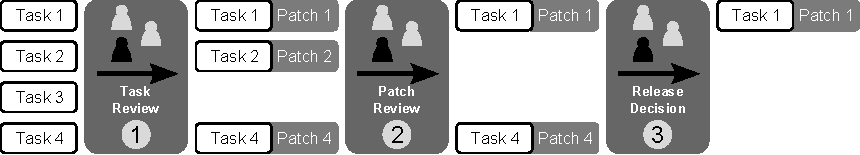
\includegraphics[width=\textwidth]{./figures/generalView}
  \caption{Main workflow followed by a task and the main points where decisions are made.}
  \label{fig:generalView}
\end{figure}

We have studied nine OSS projects where the participation is open to anyone willing to contribute, namely: Android\footnote{http://www.android.com}, GNOME\footnote{https://www.gnome.org}, 
Apache (web server) \footnote{https://www.apache.org}, Mozilla\footnote{https://www.mozilla.org}, Python\footnote{https://www.python.org}, Moodle\footnote{https://moodle.org}, EMF\footnote{https://www.eclipse.org/emf}, MoDisco\footnote{https://www.eclipse.org/modisco}. Table \ref{tab:comparative} shows a summary of the data we gathered. Next we describe the results in more detail.

\begin{table*}[t]
  \renewcommand{\arraystretch}{1.1}
  \centering
  \resizebox{\textwidth}{!}{%
    \begin{tabular}{|c|c|c|c|c|c|c|c|c|l|}\hline
    	\textbf{Project} & 
	\textbf{Organization} & 
	\textbf{Coordination} & 
	\textbf{Tracking system} & 
%	\textbf{Participation} & 
	\textbf{Task Review} & 
	\textbf{Patch Review} & 
	\textbf{Release Decision} & 
	%\textbf{Promotion} & 
	\textbf{Rules Def. / App.} &
	\begin{tabular}{c} \textbf{Roles} \end{tabular}\\ 
    \hline
 	Android &
	Hierarchy &
	Forum & 
	\begin{tabular}{c} Git \\ Gerrit \end{tabular} & 
%	Anyone & 
	\begin{tabular}{c} Yes \\ (Approver) \end{tabular} & 
	\begin{tabular}{c} Yes \\ (Verifier) \end{tabular} & 
	\begin{tabular}{c} Yes \\ (Project Lead) \end{tabular} & 
	%Selection & 
	\begin{tabular}{c} Documentation / \\ Track system\end{tabular} & 
	\begin{tabular}{l} Contributor \\ Developer \\ Verifier \\ Approver \\ Project Lead \end{tabular} \\
    \hline
        GNOME &
	Hierarchy & 
	\begin{tabular}{c} IRC \\ mailing-list \end{tabular} &
	Bugzilla &
%	Anyone &
	Yes &
	\begin{tabular}{c} Yes \\ (Bug Squad) \end{tabular} & 
	Yes &
	%Selection & 
	\begin{tabular}{c} Documentation / \\  Track System \end{tabular} & 
	\begin{tabular}{l} Contributor \\ Mentor \end{tabular} \\
%    \hline
%    	Joomla &
%	Hierarchy &
%	Forum &
%	\begin{tabular}{c} GitHub \\ Track \end{tabular} &
%	Anyone &
%	Yes &
%	\begin{tabular}{c} Yes \\ (Bug Squad) \end{tabular} & 
%	release &
%	%Selection &
%	\begin{tabular}{c} Implicit \\ (Documentation) / \\ Track System \end{tabular} & 
%	\begin{tabular}{l} Squads \end{tabular} \\
    \hline
	\begin{tabular}{c} Apache \\ Web \\ Server \end{tabular} &
	Meritocracy &
	Mailing-list &
	Bugzilla &
%	Anyone &
	\begin{tabular}{c} Yes \\ (Voting) \end{tabular} &
	\begin{tabular}{c} Yes \\ (Voting) \end{tabular} &
	\begin{tabular}{c} Yes \\ (Voting) \end{tabular} &
	% Selection &
	\begin{tabular}{c} Documentation / \\ Mailing-list \end{tabular} & 
	\begin{tabular}{l} User \\ Developer \\ Committer \\ PMC Member \\ PMC Chair \end{tabular} \\
%    \hline
%    	Linux   &
%	Hierarchy &
%	Mailing-list &
%	Git, Quilt & 
%	Anyone &
%	N/A &
%	N/A &
%	N/A &
%	%Selection &
%	\begin{tabular}{c} Implicit \\ Mailing-list \end{tabular} & 
%	\begin{tabular}{l} Any \end{tabular} \\
    \hline
    	Mozilla &
	Hierarchy & 
	\begin{tabular}{c} Forum \\ Mailing-list \\ IRC \end{tabular} &
	Bugzilla & 
%	Anyone &
	\begin{tabular}{c} Yes \\ (Module \\ Owner) \end{tabular} & 
	\begin{tabular}{c} Yes \\ (Module \\ Owner \& \\ Super-reviewers) \end{tabular} &
	\begin{tabular}{c} Yes \\ (Designated \\ Group) \end{tabular} &
	%Selection &
	\begin{tabular}{c} Documentation  / \\  Track System \& \\ Mailing-list \end{tabular} & 
	\begin{tabular}{l} User \\ Committer \\ Module Owner \\ Super-reviewer \end{tabular} \\
    \hline
    	Python &
	Hierarchy &
	\begin{tabular}{c} Mailing-list \\ IRC \\ Blogs \end{tabular} &
	\begin{tabular}{c} Mercurial \\ Roundup \end{tabular} &
%	Anyone &
	No &
	Yes (Reviewer) &
	\begin{tabular}{c} Yes \\ (Core Developer) \end{tabular} &
	%Selection & 
	\begin{tabular}{c} Documentation  / \\  Track System \end{tabular} & 
	\begin{tabular}{l} Contributor \\ Reviewer \\ Core Developer \end{tabular} \\
    \hline
    	Moodle &
	Hierarchy &
	Forum & 
	Moodle tracker &
%	Anyone & 
	\begin{tabular}{c} Yes \\ (Component \\ leads) \end{tabular} & 
	\begin{tabular}{c} Yes \\ (Developers) \end{tabular} &
	\begin{tabular}{c} Yes \\ (Component \\ Leads) \end{tabular} &
	%Selection & 
	\begin{tabular}{c} Documentation  / \\  Track System \end{tabular} & 
	\begin{tabular}{l} Users \\ Developers \\ Component Leads \\ Integrators \\ Testers \\ Manteiners \end{tabular} \\
    \hline
    	EMF &
	Hierarchy &
	Forum &
	Bugzilla & 
%	Anyone &
	\begin{tabular}{c} Yes \\ (Committer) \end{tabular} & 
	\begin{tabular}{c} Yes \\ (Committer) \end{tabular} & 
	\begin{tabular}{c} Yes \\ (Project Leader) \end{tabular} & 
	%Selection &
	\begin{tabular}{c} Documentation  / \\  Track System \end{tabular} & 
	\begin{tabular}{l} User \\ Contributor \\ Committer \\ Project Leader \end{tabular} \\
    \hline
    	MoDisco &
	Hierarchy &
	Forum &
	Bugzilla &
%	Anyone & 
	\begin{tabular}{c} Yes \\ (Committer) \end{tabular} &
	\begin{tabular}{c} Yes \\ (Committer) \end{tabular} &
	\begin{tabular}{c} Yes \\ (Committers) \end{tabular} &
	%Selection &
	\begin{tabular}{c} Documentation  / \\  Track System \end{tabular} & 
	\begin{tabular}{l} User \\ Contributor \\ Committer \\ Project Leader \end{tabular} \\
    \hline
  \end{tabular}}
  \caption{Comparison of how OSS systems are governed.}
  \label{tab:comparative}
\vspace{-0.25cm}
\end{table*}

\vspace{0.15em}
\noindent \textbf{Organization}. The organization followed by a project summarizes its main development philosophy. The great majority of analyzed projects follow a hierarchical scheme, thus meaning that there exist several hierarchical levels in the groups of users collaborating in the development (e.g., leaders, contributors, users, etc.). Thus, there are several roles (see the corresponding feature below) which a user can belong to. A good example is the Android project, where each role has assigned a particular function in the process (e.g., \textit{approvers} approve tasks, \textit{verifiers} review patches, etc.) supporting the project leader. On the other hand, Apache differs from the others by using a meritocracy organization where users can gain merits as they contribute to the project. 

\vspace{0.15em}
\noindent \textbf{Coordination}. This feature includes the main tools used to help users to collaborate during the development process. As can be seen, mailing-list and forums are the main tools used. Note that even though these tools are useful to keep in touch with the rest of developers, they are normally used to apply some governance rules as well, which goes beyond the original purpose of those tools. This is the case of Apache, which uses a mailing-list to vote which issues/bugs should be implemented/fixed next.

\vspace{0.15em}
\noindent \textbf{Tracking system}. The managament of tasks is performed by tracking systems, Bugzilla being the most popular one. Interestingly enough, tracking systems are also used as a forum-like tool to discuss possibles tasks which are not mature enough to be considered as real issues. For instance, in the GNOME project, some tasks\footnote{http://felipec.wordpress.com/2011/09/23/no-gnome-doesnt-want-user-feedback-how-i-argued-in-favor-of-voting-in-bugzilla-and-got-banned-as-a-result} in Bugzilla are used to openly discuss possible changes in the development strategy.

%  \item \textbf{Participation}. In general, in OSS systems, anyone is able to take part in the development, i.e. it is not necessary to be an official developer to inform new issues or bugs. 

\vspace{0.15em}
\noindent \textbf{Task review}. Once a task (i.e., issue/bug) is notified, it can be reviewed to be accepted or rejected. Except for Python, where all the task are accepted and only reviewed if they include the corresponding patch, the rest of the projects have a decision process to accept or reject the task proposal. In general, the decision process is made by either the leader (e.g., component leaders in Moodle) or by unanimous agreement if there are several leaders (e.g., in big Eclipse-based projects such as EMF).

\vspace{0.15em}
\noindent \textbf{Patch review}. Tasks have attached the corresponding patch implementing the improvement (if it is an issue) or the fix (if it is a bug). Before incorporating the patch into the product, it is possible to perform a revision and test to check the quality of the patch. All the analyzed projects include a review process which analyzes the patch and eventually decides its acceptance or rejection.

\vspace{0.15em}
\noindent \textbf{Release Decision}. As the tasks and the corresponding patches are accepted, new software product releases have to be published. In the vast majority of analyzed projects, the decision of selecting when to perform the release and which tasks should be incorporated normally is taken by the product/component leader or by unanimous agreement when there are several leaders. The only exception is the decision process for Apache, where a ballot takes place.

\vspace{0.15em}
\noindent \textbf{Governance rule definition and application}. This feature shows how governance rules are defined and applied. In general, none of the projects explictly defines these rules, and the result of their application is scattered througout the management systems (i.e., track systems or mailing-lists).

%  \item \textbf{Promotion}. This feature describes how people can gain specific roles in the community. All the projects analyzed applies a selection process where a leader chooses who should change the role. Only in the Apache community, the selection process is performed by voting.

\vspace{0.15em}
\noindent \textbf{Roles}. The users collaborating in the development are classified according to a set of roles. All the analyzed projects include both the role of developer (also known as contributor or commiter), who can commit changes into the source code repository of the project and the corresponding role for leaders (also known as owners or chairs).

In summary, most projects are hierarchical where a group of contributors are driven by a leader (or a set of leaders) who normally decides which tasks should be completed first. Patches are normally reviewed and tested by contributors while the product release is decided by a leader group as well. Thus, the resulting governance rules are mainly controlled by the group of leaders, who can decide how the software product should evolve. When there is a group of leaders, the decision is normally made by unanimous agreement and normally using tools such as email, mailing-lists or forums. 

The development of Apache web server is the main exception. The project is governed by a vote-based strategy where all the contributors can decide which tasks should be accepted and which ones should be included into the final release. It is important to note that although anyone can vote, only the votes from contributors are binding, the rest are helpful to see the general opinion of the community. The project also establishes how the voting should be performed. Thus, if the task involves changes in the source code, the voting should unanimously agree to make the change and at least three votes must be casted. Otherwise, if the change does not involve code, a majority of positives votes (and at least three) are required. Moreover, any negative vote must include the corresponding rationale, which can therefore help to solve the disagreement.

Interestingly enough, in all the analyzed projects it was not trivial for us to discover the governance rules being applied since the available information was scarce and normally scattered among the documentation of the project. In fact, some projects such as GNOME recommend to be patient since it can take a long time to become a contributor. Potential contributors are therefore required to observe existing mailing lists, conversations on IRC, etc. to discover the way of working in the project. 

Moreover, the result of the application of these rules is directly updated in the tracking systems, where normally there is no tracking information that helps to clarify later on why that decision was taken nor the possible discussion threads (maybe taken place outside the tracking systems, e.g., by chat or email as it is the case for smaller projects such as MoDisco) among the leaders that lead to that decision. 

Clearly, making explicit the governance rules followed in a project could help the developer community to understand and apply those rules as part of their daily development activities. Next sections describe our proposal to tackle this problem.

